\documentclass[12pt,a4paper,bibliography=totocnumbered,listof=totocnumbered]{scrartcl}
\usepackage[ngerman]{babel}
\usepackage[utf8]{inputenc}
\usepackage{amsmath}
\usepackage{amsfonts}
\usepackage{amssymb}
\usepackage{graphicx}
\usepackage{fancyhdr}
\usepackage{tabularx}
\usepackage{geometry}
\usepackage{setspace}
\usepackage[right]{eurosym}
\usepackage[printonlyused]{acronym}
\usepackage{subfig}
\usepackage{floatflt}
\usepackage[usenames,dvipsnames]{color}
\usepackage{colortbl}
\usepackage{paralist}
\usepackage{array}
\usepackage{titlesec}
\usepackage{parskip}
\usepackage[right]{eurosym}
\usepackage{picins}
\usepackage[subfigure,titles]{tocloft}
\usepackage[pdfpagelabels=true]{hyperref}
\usepackage[inline]{enumitem}
\usepackage[section]{placeins}

\usepackage{listings}
\lstset{basicstyle=\footnotesize, captionpos=b, breaklines=true, showstringspaces=false, tabsize=2, frame=lines, numbers=left, numberstyle=\tiny, xleftmargin=2em, framexleftmargin=2em}
\makeatletter
\def\l@lstlisting#1#2{\@dottedtocline{1}{0em}{1em}{\hspace{1,5em} Lst. #1}{#2}}
\makeatother

\geometry{a4paper, top=27mm, left=30mm, right=20mm, bottom=35mm, headsep=10mm, footskip=12mm}

\hypersetup{unicode=false, pdftoolbar=true, pdfmenubar=true, pdffitwindow=false, pdfstartview={FitH},
	pdftitle={Entwurf und Implementierung einer Chrome Extension zur automatischen Anreicherung von Webseiten mit kulturellen Inhalten},
	pdfauthor={Mathias Möller},
	pdfsubject={Bachelorarbeit},
	pdfcreator={\LaTeX\ with package \flqq hyperref\frqq},
	pdfproducer={pdfTeX \the\pdftexversion.\pdftexrevision},
	pdfkeywords={Bachlorarbeit},
	pdfnewwindow=true,
	colorlinks=true,linkcolor=black,citecolor=black,filecolor=magenta,urlcolor=black}
\pdfinfo{/CreationDate (D:20110620133321)}

\begin{document}

\titlespacing{\section}{0pt}{12pt plus 4pt minus 2pt}{-6pt plus 2pt minus 2pt}

% Kopf- und Fusszeile
\renewcommand{\sectionmark}[1]{\markright{#1}}
\renewcommand{\leftmark}{\rightmark}
\pagestyle{fancy}
\lhead{}
\chead{}
\rhead{\thesection\space\contentsname}
\lfoot{Entwurf und Implementierung einer Chrome Extension zur automatischen\newline Anreicherung von Webseiten mit kulturellen Inhalten}
\cfoot{}
\rfoot{\ \linebreak Seite \thepage}
\renewcommand{\headrulewidth}{0.4pt}
\renewcommand{\footrulewidth}{0.4pt}

% Vorspann
\renewcommand{\thesection}{\Roman{section}}
\renewcommand{\theHsection}{\Roman{section}}
\pagenumbering{Roman}

% ----------------------------------------------------------------------------------------------------------
% Titelseite
% ----------------------------------------------------------------------------------------------------------
\thispagestyle{empty}
\begin{center}
	
\includegraphics[scale=0.3]{Bilder/uni_passau.png}\\
	\vspace*{2cm}
	\Large
	\textbf{Fakultät für}\\
	\textbf{Informatik und Mathematik}\\
	\vspace*{2cm}
	\Huge
	\textbf{Bachelorarbeit}\\
	\vspace*{0.5cm}
	\large
	über das Thema\\
	\vspace*{1cm}
	\textbf{Entwurf und Implementierung einer Chrome Extension zur automatischen Anreicherung von Webseiten mit kulturellen Inhalten}\\
	\vspace*{2cm}
	
	\vfill
	\normalsize
	\newcolumntype{x}[1]{>{\raggedleft\arraybackslash\hspace{0pt}}p{#1}}
	\begin{tabular}{x{6cm}p{7.5cm}}
		\rule{0mm}{5ex}\textbf{Autor:} & Mathias Möller\newline moellerm@fim.uni-passau.de \\ 
		\rule{0mm}{5ex}\textbf{Prüfer:} & Prof. Dr. Granitzer \\ 
		\rule{0mm}{5ex}\textbf{Abgabedatum:} & 26.08.2015 \\ 
	\end{tabular} 
\end{center}
\pagebreak

% ----------------------------------------------------------------------------------------------------------
% Abstract
% ----------------------------------------------------------------------------------------------------------
\setcounter{page}{1}
\onehalfspacing
\titlespacing{\section}{0pt}{12pt plus 4pt minus 2pt}{2pt plus 2pt minus 2pt}
\rhead{KURZFASSUNG}
\section{Kurzfassung}
Lorem ipsum dolor sit amet, consetetur sadipscing elitr, sed diam nonumy eirmod tempor invidunt ut labore et dolore magna aliquyam erat, sed diam voluptua. At vero eos et accusam et justo duo dolores et ea rebum. Stet clita kasd gubergren, no sea takimata sanctus est Lorem ipsum dolor sit amet. Lorem ipsum dolor sit amet, consetetur sadipscing elitr, sed diam nonumy eirmod tempor invidunt ut labore et dolore magna aliquyam erat, sed diam voluptua. At vero eos et accusam et justo duo dolores et ea rebum. Stet clita kasd gubergren, no sea takimata sanctus est Lorem ipsum dolor sit amet.

\pagebreak

% ----------------------------------------------------------------------------------------------------------
% Verzeichnisse
% ----------------------------------------------------------------------------------------------------------
% TODO Typ vor Nummer
\renewcommand{\cfttabpresnum}{Tab. }
\renewcommand{\cftfigpresnum}{Abb. }
\settowidth{\cfttabnumwidth}{Abb. 10\quad}
\settowidth{\cftfignumwidth}{Abb. 10\quad}

\titlespacing{\section}{0pt}{12pt plus 4pt minus 2pt}{2pt plus 2pt minus 2pt}
\singlespacing
\rhead{INHALTSVERZEICHNIS}
\renewcommand{\contentsname}{II Inhaltsverzeichnis}
\phantomsection
\addcontentsline{toc}{section}{\texorpdfstring{II \hspace{0.35em}Inhaltsverzeichnis}{Inhaltsverzeichnis}}
\addtocounter{section}{1}
\tableofcontents
\pagebreak
\rhead{VERZEICHNISSE}
\listoffigures
\pagebreak
%\listoftables
%\pagebreak

% ----------------------------------------------------------------------------------------------------------
% Inhalt
% ----------------------------------------------------------------------------------------------------------
% Abstände Überschrift
\titlespacing{\section}{0pt}{12pt plus 4pt minus 2pt}{-6pt plus 2pt minus 2pt}
\titlespacing{\subsection}{0pt}{12pt plus 4pt minus 2pt}{-6pt plus 2pt minus 2pt}
\titlespacing{\subsubsection}{0pt}{12pt plus 4pt minus 2pt}{-6pt plus 2pt minus 2pt}

% Kopfzeile
\renewcommand{\sectionmark}[1]{\markright{#1}}
\renewcommand{\subsectionmark}[1]{}
\renewcommand{\subsubsectionmark}[1]{}
\lhead{Kapitel \thesection}
\rhead{\rightmark}

\onehalfspacing
\renewcommand{\thesection}{\arabic{section}}
\renewcommand{\theHsection}{\arabic{section}}
\setcounter{section}{0}
\pagenumbering{arabic}
\setcounter{page}{1}

\section{Einleitung und Motivation}
Suchmaschinen gehören heutzutage zu den meistbesuchten Seiten im Internet. Google\footnote{https://www.google.com/} ist mit 2.000.000.000.000 Suchanfragen pro Jahr (TODO: Quelle) nicht nur die beliebteste Suchmaschine, sondern auch die meist besuchte Seite im Internet. Auch die chinesische Suchmaschine Baidu\footnote{http://www.baidu.com/} ist in den oberen fünf Plätzen vertreten \cite{alexa}. 
\begin{itemize}
	\item Auf XX\% der Webseiten wird über eine Suchmaschine zugegriffen
	\item Menschen holen Informationen über Suchmaschinen, nicht mehr aus Bibliotheken oder Lexika 
	\item Woher Quellen?
\end{itemize}
Um so mehr sie an Bedeutung gewinnen, umso größer ist der Bedarf an bessern Suchmaschinen \cite{lawrence2000context}.

Doch der Funktionsumfang klassischer Suchmaschinen ist begrenzt. Sie können den Kontext des Benutzers in ihren Queries? nicht miteinbeziehen. Weiterhin verlangen sie vom Nutzer, seine gegenwärtige Arbeit einzustellen, die Webseite der Suchmaschine aufzurufen und eine Suchanfrage zu formulieren. So wird die Konzentration auf den eigentlichen Arbeitsschritt gestört. Im Schnitt sind nur 67\% der Suchanfragen an Google erfolgreich (TODO: Quelle). Das heißt in circa einem Drittel der Fälle bleibt der Aufruf der Suchmaschine ohne die erwarteten Erfolge. Zu der verlorenen Zeit addiert sich auch noch die Zeit, die der Nutzer braucht um sich seine Arbeit wieder ins Kurzzeitgedächtnis zu holen.

Um diesen Problemen entgegen zu wirken wurden neue Wege zur Informationsgewinnung entwickelt. Eine Möglichkeit sind so genannte Just-in-time Information Retrieval Agents (JITIR-Agents) \cite{rhodes2000just}. Sie beobachten im Hintergrund den Kontext des Benutzers und versuchen aus den so erhaltenen Informationen eine Suchanfrage an eine Datenbank oder ein Recommender-System zu schicken. Die gewonnenen Informationen werden dann möglichst unaufdringlich dem Benutzer angezeigt. Er kann sich nun entscheiden diese Informationen genauer zu betrachten oder mit seiner Arbeit fortzufahren. Die kognitive Belastung bleibt hierbei sehr gering. JITIR-Agents reduzieren auf diese Weise enorm den Aufwand Informationen zu finden \cite{rhodes2000just}.

Durch ihre Funktionsweise sind sie jedoch nicht so exakt wie klassische Suchmaschinen, da sie nur ``erraten'' können, was den Benutzer gerade interessiert. Wenn ein Benutzer einer genaue Vorstellung von der Suchanfrage oder den Ergebnissen hat, haben klassische Suchmaschinen Vorteile gegenüber den JITIR-Agents \cite{rhodes2000just}.

Ein weiteres Problem des Internets ist es, dass die Standards, die die simple und leicht skalierbare Architektur des Netzwerks ermöglichen, den Einsatz von fortgeschritteneren Hypermedia-Technologien verhindern \cite{bouvin1999unifying}. Eine Möglichkeit, das Internet um Funktionen zu erweitern ist Web Augmentation (WA). Diaz \cite{diaz2012understanding} beschreibt WA als den Versuch, statt eine neue Technologie zu entwickeln, neue Funktionalität auf eine gerenderte Webseite zu setzen:
\begin{quote}
In some sense, WA is to the Web what Augmented Reality is to the physical world: layering relevant content/layout/navigation over the existing Web to customize the user experience. \cite{diaz2012understanding}
\end{quote}
Solche WA-Tools interagieren mit einem Web Server, Http-Proxy oder dem Browser der Nutzers, um so Inhalte oder Navigationselemente direkt in die angezeigte Webseite einzufügen. Auf diese Weise erlauben sie es, die limitierten Möglichkeiten des World Wide Webs zu Gunsten des Nutzers anzureichern (QUelle: Kennth anderson oder Bouvin).

Ein Beispiel für ein solches WA-Tool sowie für ein JITIR System ist das EEXCESS Chrome Plugin\footnote{http://eexcess.eu/results/chrome-extension/}. Es analysiert die aktuell besuchten Seiten des Nutzers und schlägt ihm auf Grund der erlangten Daten am Rand des Browser-Fensters weiterführende Quellen aus der Europeana-Datenbank\footnote{http://www.europeana.eu/portal/} vor.

Ziel dieser Bachelorarbeit ist es, auf Basis des EEXCESS Plugins ein Chrome Plugin zu entwerfen und zu implementieren, welche eine Webseite in einzelne Paragraphen aufteilt und zu jedem dieser Paragraphen kulturelle Inhalte der Europeana-Datenbank vorschlägt. Dabei soll das Design des Plugins helfen, die bei der in Kapitel 5 erläuterten Evaluierung des EEXCESS Plugins aufgetauchten Probleme zu beheben und Schwachstellen zu verbessern.

Im zweiten Teil dieser Arbeit wird auf vergleichbare Technologien eingegangen und ihre Gemeinsamkeiten und Unterschiede zu diesem Projekt. Anschließend wird das Konzept und die Implementierung des Projekts beschrieben und das Ergebnis evaluiert. Der sechste Teil der Ausarbeitung widmet sich Möglichkeiten für zukünftige Projekte und Verbesserungen. Zuletzt wird ein Fazit gezogen und die Ergebnisse der Arbeit analysiert.
\section{Related Work}
Rhodes \cite{rhodes2000just} definiert JITIR-Agents als eine Klasse von Programmen, die dem Benutzer weiterführende Informationen basierend auf seinem lokalen Kontext anzeigen. Dabei beschränkt sich der überwachte Kontext meist auf die virtuelle Umgebung des Benutzers, wie E-Mail, Webseiten und geöffnete Dokumente. Als Kerneigenschaften von JITIR-Agents nennt Rhodes Selbstständigkeit, die Fähigkeit Informationen in einer leicht zugänglichen und gleichzeitig unaufdringlichen Weise darzustellen und das Bewusstsein über den Kontext des Benutzers \cite{rhodes2000thesis}.
Das im Zuge dieser Bachelorarbeit entworfene Programm (im Folgenden als Jarvis bezeichnet) erfordert vom Nutzer die explizite Aufforderung um nach Informationen zu suchen. Gründe für diese Entscheidung werden im dritten Kapitel näher betrachtet. Trotz dieses Widerspruchs zu Rhodes Definition lässt sich Jarvis am besten mit dieser Klasse von Programmen vergleichen. Warum diese Klassifizierung zutrifft wird im folgenden Abschnitt beschrieben.

\subsection{Unterschiede und Gemeinsamkeiten zu JITIR-Agents}
Studien haben gezeigt, dass schon eine kleine Steigerung des Aufwands, der betrieben werden muss um eine Aufgabe zu erfüllen, dazu führen kann, dass man die Aufgabe gar nicht erst ausführt \cite{rhodes2000just}. Laut Miller reicht für die meisten Aufgaben eine Antwortverzögerung von mehr als zwei Sekunden aus, um die Nutzungshäufigkeit des dazugehörigen Programms zu vermindern \cite{miller1968response}. Längere Zeitintervalle erschweren es, den Kontext der gerade ausgeführten Aufgabe und die übergeordneten Aufgaben im Kurzeitgedächtnis zu behalten. Nun wird der Fall betrachtet, dass das Lesen einer Webseite unterbrochen wird, um eine Suche mit einer Suchmaschine durchzuführen. Die eigentliche Aufgabe behält der Nutzer im Kurzzeitgedächtnis. Je länger die Suche dauert und je mehr er sich dazu von seiner eigentlichen Arbeit distanzieren muss, desto schwerer wird es wieder zur Hauptaufgabe zurück zu kehren. Wenn der Exkurs zur Suchmaschine schwerer wiegt ist als die Güte der erwarteten Resultate wird die Suche nicht durchgeführt \cite{rhodes2000just}.

Dieses Problem wird versucht mit JITIR-Agents zu beheben. Durch ihre proaktive Arbeitsweise muss der Nutzer seine Tätigkeit nicht mehr unterbrechen, sondern nur noch entscheiden ob er weiter Informationen sehen möchte oder nicht \cite{rhodes2000just}. Beim Entwurf von Jarvis wurde entschieden, dass das Programm nicht völlig eigenständig nach Informationen sucht, sondern nur die Webseite in seine Paragraphen aufteilt. Der Nutzer kann dann entscheiden, ob er zu einem Paragraphen eine Suche durchführen möchte und diese dann per Klick starten. Wie bei einem JITIR-Agent wird die Suchanfrage automatisch aus den gewonnenen Kontextinformationen generiert. Da die Suche innerhalb weniger Millisekunden ausgelöst werden kann und sich der Nutzer dazu nicht von seiner eigentlichen Aufgabe distanzieren muss, bleibt die kognitive Belastung sehr gering. Allerdings entsteht auch so der Nachteil, den Jarvis mit JITIR-Agents gemein hat: Sie nutzen alle gefunden Informationen für ihre Suchanfragen und können nicht zwischen relevanten und unwichtigen Suchwörtern unterscheiden \cite{rhodes2000margin}. Automatisch gebaute Suchanfragen sind deshalb weniger exakt als Menschen-generierte \cite{rhodes2000just}. Um dem entgegen zu wirken hat der Benutzer von Jarvis im Nachhinein noch die Möglichkeit, die Suche anzupassen und erneut abzuschicken.

Die zweite von Rhodes beschriebene Eigenschaft von JITIR-Agents, die Fähigkeit Informationen in einer leicht zugänglichen und gleichzeitig unaufdringlichen Wiese darzustellen, hat auch beim Entwurf von Jarvis eine bedeutende Rolle gespielt. Für die Darstellung der Ergebnisse muss ein Mittelwert gefunden werden. Die zusätzlichen Elemente sollen den Benutzer nicht unnötig ablenken, allerdings will man die Seite um möglichst reichhaltige Informationen erweitern \cite{rhodes2000margin}. Wie diese Problematik im Falle von Jarvis gelöst wurde wird im Implementierungs-Teil dieser Arbeit beschrieben.

Jarvis analysiert die geöffnete Webseite und teilt diese in Paragraphen ein. Wie JITIR-Agents ist er sich also über den lokalen Kontext des Benutzers bewusst und wertet diesen aus. Die dritte Voraussetzung für JITIR-Agents ist somit erfüllt.

Trotz der eingeschränkten Selbstständigkeit lässt sich Jarvis folglich am besten mit denen von Rhodes beschriebenen Programmen vergleichen. Auf diese Erkenntnis aufbauend wird nachfolgend Jarvis mit existierenden Implementierungen von JITIR-Agents verglichen.

\subsection{Vergleich mit existierenden JITIR-Agents}
Es wurden einige JITIR-Agents in der Vergangenheit implementiert, die zwar aus technischer Hinsicht nicht mehr aktuell sind, die sich jedoch durch ihre genaue Untersuchung und Auswertung gut Vergleichen lassen.

 	\subsubsection{Remembrance Agent}
 	Der Remembrance Agent (RA) ist ein in den UNIX Texteditor EMACS-19 integriertes Programm, welches eine Liste von Dokumenten anzeigt, die für den Nutzer interessant seien könnten \cite{rhodes2000thesis}. Die Informationen für die Vorschläge bezieht der RA aus der gerade geöffneten Datei. Wie Jarvis teilt er das Dokument in Bereiche ein, die er danach analysiert. Allerdings sind die Bereiche in diesem Fall keine Paragraphen sondern verschieden große ``Räume'' in denen er sucht. Von der Position des Cursors ausgehend untersucht er die nächsten zehn, die nächsten 50 und die nächsten 1000 Wörter des Dokuments und sucht zu jedem passende Vorschläge \cite{rhodes1996remembrance}. Die Vorschläge werden von einem Information Retrieval Programm im Hintergrund generiert, welches die Suchanfragen an verschiedene, vom Nutzer konfigurierbare Datenbanken schickt. Genannte Datenbanken sind persönliche Email-Verzeichnisse, persönliche Notizen oder Datenbanken mit wissenschaftlichen Arbeiten.

 	Die gefundenen Ergebnisse werden dem Nutzer dann am unteren Fensterrand dargestellt. Mehrere Zeilen präsentieren die Vorschläge mit der höchsten Relevanz. Je nach Art der Quellen werden verschiedene Informationen angezeigt. So werden zum Beispiel bei wissenschaftlichen Arbeiten der Autor, das Datum und der Titel angezeigt und bei Zeitungsartikeln nur Herausgeber, Überschrift und Datum \cite{rhodes2000just}. Dieses Design ermöglicht eine unaufdringliche Darstellung der Vorschläge, die leicht überblickt werden kann aber den Nutzer nicht von seiner Arbeit ablenkt \cite{rhodes1996remembrance}. Per Klick kann sich der Nutzer die Schlagwörter anzeigen lassen, die für das jeweilige Ergebnis verantwortlich sind \cite{rhodes2000thesis}. Mit einer Tastenkombination und der Zeilennummer des Vorschlags kann er sich das dazugehörende, vollständige Dokument anzeigen lassen. Weiterhin hat der Nutzer die Möglichkeit, eine eigene Suchanfrage einzugeben um so explizit nach Inhalten zu suchen \cite{rhodes1996remembrance}.

 	Mit Hilfe einer Nutzer-Evaluation konnte gezeigt werden, dass der RA nicht nur eine Alternative zu klassischen Suchmaschinen darstellt, sondern in vielen Bereichen sogar besser abscheidet. Durch die Nutzung fanden die Tester mehr relevante Dokumente zum geforderten Themengebiet und die anschließende Umfrage schnitt der RA besser ab als die der Kontrollgruppe zur Verfügung gestellte Suchmaschine \cite{rhodes2000just}.

 	\subsubsection{Watson}
 	Watson ist ein weiteres Beispiel für JITIR-Agents\footnote{Die Entwickler beschreiben das System als ``Information Management Assistant'', die Bedeutung ist jedoch ähnlich.}. Er überwacht die Benutzung von Textverarbeitungs- und Textdarstellungsprogrammen wie Microsoft Word, Microsoft Internet Explorer oder Netscape Navigator \cite{budzik1999watson}. Dazu werden sogenannte ``Application Adapter'' benutzt, die sich mit der jeweiligen Software verbinden um so an den Inhalt der angezeigten oder bearbeiteten Dokumente zu gelangen \cite{budzik2000user}. Die erlangten Informationen werden an Watson weitergegeben, welcher versucht eine passende Quelle aufgrund dieser Daten auszuwählen. Ein weiterer Prozess versucht zu erkennen, ob der Nutzer Bedarf an zusätzlichen Informationen hat. Trifft das zu, wird eine Anfrage an die ausgewählte Quelle/die ausgewählten Quellen geschickt. Die Ergebnisse werden dann gruppiert und in einem separaten Fenster angezeigt \cite{budzik1999watson}.

 	Auch bietet Watson die Möglichkeit, eine Suchanfrage direkt einzugeben. Die Anfrage des Nutzers wird daraufhin mit der automatisch erstellten, kontextabhängigen Anfrage kombiniert um so möglichst relevante Ergebnisse zu liefern \cite{budzik2000user}. Weiterhin werden atomare Bausteine, wie Adressen erkannt. Dem Nutzer wird dann ein Knopf angezeigt, über den er zu einer passenden Darstellung des Bausteins gelangt. Im Falle einer Adresse würde er zum Beispiel zu einer Karte weitergeleitet werden, in der die Adresse angezeigt wird.

 	Evaluationen haben gezeigt, dass die von Watson vorgeschlagenen Dokumente in fünf von zehn Fällen relevant waren. Die Kontrollgruppe, welche die Suche manuell mit Alta Vista\footnote{\url{http://de.wikipedia.org/wiki/AltaVista}} durchführen mussten (Watson benutzte als Quelle auch Alta Vista), kamen im Schnitt auf nur drei relevante Ergebnisse. Schlussendlich erzielte Watson bessere Ergebnisse als die Kontrollgruppe in 15 von 19 Fällen \cite{budzik1999watson}.

 	\subsubsection{EEXCESS Chrome Plugin}
 	Das von EEXCESS\footnote{\url{http://eexcess.eu/}} entwickelte Chrome Plugin\footnote{\url{http://eexcess.eu/results/chrome-extension/}} benutzt JITIR Mechanismen um kulturelle Inhalte der Europeana Datenbank für den Nutzer leichter zugänglich zu machen. Die Software analysiert die aktuelle Webseite oder gegebenenfalls einen selektierten Paragraphen innerhalb dieser Seite und die gewonnenen Daten werden in Form einer Anfrage an Europeana geschickt \cite{schlottererweb}. Die personalisierten Resultate werden dem Benutzer am Rande des Browserfensters in einem separierten Bereich angezeigt.

\subsection{Interactive Query Construction}
Ein System welches Interactive Query Construction verwendet, ist das von Russel et al. entwickelte NITELIGHT \cite{russell2008nitelight}. Es unterstützt Nutzer bei der Erstellung und Anpassung von Suchanfragen auf Basis der SPARQL \cite{sparql} Abfragesprache. Das in Java entwickelte Programm erlaubt es dem Nutzer über eine graphische Oberfläche interaktiv semantische Anfragen zu bauen. Dazu werden ihm graphische Elemente zur Verfügung gestellt, die auf Konstrukten der Abfragesprache basieren \cite{russell2008nitelight}. Die in Jarvis verwendete Interactive Query Construction ist stark vereinfacht und ermöglicht es dem Nutzer lediglich, die automatisch generiert Anfrage zu erweitern oder irrelevante Schlüsselwörter zu entfernen. Jedoch ermöglicht die Nutzung dieser Methodik eine leichte Erweiterbarkeit um Funktionen zur Verbesserung der Ergebnisgüte wie zum Beispiel ``Relevance Feedback''. Darauf wird in Kapitel \ref{sec:futureWork} genauer eingegangen. 

\subsection{Text Retrieval Algorithmen}
 		Term Frequency/Inverse Document Frequency algorithm,
 		Text rank
\section{Konzept}
 Wie auch bei der von EEXCESS entwickelten Extension fiel auch bei Jarvis die Wahl auf eine Chrome Extension. Google Chrome hat mit 40\% den größten Marktanteil unter Web Browsern und durch die Ähnlichkeit der Extension Architektur von Chrome zu anderen Browsern kann die Anwendung im Nachhinein leicht auf diese übertragen werden \cite{schlottererweb}. Per ``JavaScript Injection'' kann in diesen Architekturen das Aussehen und Verhalten der Seite verändert und neue Funktionalität hinzugefügt werden \cite{schlottererweb}.

 Beim Entwurf von Jarvis wurde sich am Design von JITIR-Agents orientiert. Trotzdem sucht Jarvis nicht proaktiv nach Ergebnissen, sondern erst nach einer Interaktion des Users. Zum einen entstehen durch die Nutzung der Europeana API technische Limitierungen. Für jeden API-Key lässt Europeana pro Tag nur 10.000 Anfragen zu \cite{europlimit}. Dieser API-Key wird von allen installierten Jarvis Extensions genutzt. Da in jeder geöffneten Webseite für jeden gefundenen Paragraphen eine eigene Anfrage an die Europeana API gesendet werden würde, wäre dieses Limit ab einer gewissen Anzahl von Nutzern schnell überschritten. Zum anderen kann der User so entscheiden, ob er zum jeweiligen Paragraphen weitere Informationen erhalten möchte oder nicht. Möchte er dass nicht, wird seine Aufmerksamkeit auch nicht durch das erscheinen von Ergebnissen gestört. Der letzte Grund, der zu dieser Entscheidung geführt hat, ist, dass der User sich auf diese Weise seine Suchanfrage selber erstellen kann, bevor diese abgeschickt wird. Entsteht beim Lesen eines Absatzes ein Bedarf auf spezifische Informationen, kann der User die Anfrage direkt über dem Absatz einfügen oder sie interaktiv zusammenbauen. Die Resultate dieser Anfrage haben mit hoher Wahrscheinlichkeit eine höhere Relevanz als die von einer automatisch generierten \cite{rhodes2000just}.

 Der Entwurf der Extension lässt sich in vier Ziele einteilen:
 \begin{enumerate*}
 	\item Die Anzeige der Ergebnisse
  	\item Die Erklärung der Suchanfragen Generierung
 	\item Das Anpassen der Suchanfrage durch den User
 	\item Die Verbesserung der Ergebnisgüte.
\end{enumerate*}
Auf diese Ziele wird im folgenden genauer eingegangen.

 \subsection{Anzeige der Ergebnisse}
 Nachdem eine Anfrage an die Europeana API gesendet wurde und die Ergebnisse beim Client angekommen sind, müssen diese dargestellt werden. Der User soll leicht erkennen können, welche der ihm angezeigten Elemente aus der ursprünglichen Webseite stammen und welche durch die Extension hinzugekommen sind. Aus diesem Grund wurde bei Jarvis ein einheitliches und buntes Design gewählt. So setzt sich die Anwendung deutlich von den meisten Webseiten ab. Auch soll eine enge Bindung zwischen den Ergebnissen und dem dazugehörigen Paragraphen geschaffen werden. Um das zu erreichen, werden die durch die Paragraphen-Erkennung gefundenen Textpassagen hervorgehoben und die Ergebnisse direkt bei den jeweiligen angezeigt.

 Weiterhin ist es wichtig, einen Mittelwert zu finden, was die Menge der angezeigten Informationen betrifft. Zu viele Informationen auf einmal können den User ablenken. Auf der anderen Seite ist es das Ziel dem User eine möglichst reichhaltige alternative Informationsquelle zu liefern \cite{rhodes2000margin}. Rhodes empfiehlt hierfür ein Ramping Interface \cite{rhodes2000just}. Hierbei werden die Informationen in Stufen aufgeteilt. Jede Stufe liefert etwas mehr Informationen als die vorherige. Auf diese Weise kann der User entscheiden ob er mehr Informationen sehen möchte und daraufhin auf die nächste Stufe gehen oder nicht.

 Jarvis zeigt nach einer erfolgreichen Suche zunächst nur die Anzahl der gefundenen Ergebnisse an. Diese Anzeige ist aufgeteilt in Anzahl der textuellen Ergebnisse, der gefundenen Bilder sowie der gefundenen Audio- und Videoquellen. Durch Auswählen einer der drei Kategorien werden in einem sich über dem Paragraphen öffnenden Fenster eine Liste mit Titel und Vorschaubild der Ergebnisse angezeigt. Die Liste ist absteigend nach der Relevanz sortiert, die Europeana in Form eines Relevance Scores mitliefert. Durch ändern des Tabs kann hier zwischen den Kategorien gewechselt werden.
 Durch einen Klick auf den Titel oder das Bild eines Listeneintrages kann der User die entsprechende Quelle aufrufen. Bewegt er bei Text- oder Audio-/Videoquellen den Cursor über das Miniaturbild eines Ergebnisses, werden ihm weitere Informationen angezeigt. Unter anderem die Sprache, die Nutzungsrechte und der Relevance Score der Quelle. Da bei Bildquellen die Metadaten nicht so wichtig sind wie das Bild selber, werden sie in einer Gitter-Liste angezeigt. Die Listen-Elemente bestehen aus einem mittelgroßen Vorschaubild sowie dem Titel des Bildes. Durch klicken gelangt der User zur Quelle des Bildes. Weitere Informationen werden nicht angezeigt, da sie für die Entscheidung die Quelle aufzurufen in den meisten Fällen unwichtig sind.

 \subsection{Erklärung der Suchanfragen Generierung}
 \label{ssec:suchanfragenGenerierung}
 Für den User soll es einfach zu erkennen sein, wie die Ergebnisse zustande gekommen sind. Dafür ist es wichtig, dass er sieht aus welchen Suchbegriffen die Anfrage zusammengesetzt wurde. Nach dem Auslösen der Suchfunktion der Extension werden die Schlagwörter, die aus diesem Paragraphen extrahiert wurden, über diesem angezeigt. Diese Anzeige erlaubt auch die Manipulation der Suchanfrage. Weiterhin werden die gefundenen Schlagwörter im Text hervorgehoben.

 \subsection{Anpassen der Suchanfrage durch den User}
 Da automatisch generierte Suchanfragen nicht immer die gewünschten Ergebnisse liefern, kann der User die Suchanfrage selber erstellen oder die generierte manipulieren. Dazu kann er Wörter aus dem Text hinzufügen oder eigene eingeben. Aus der bestehenden Anfrage kann er unpassende oder mehrdeutige Suchbegriffe entfernen. Durch diese Interaktionsmöglichkeiten soll das Programm so intuitiv wie möglich gestaltet werden um Nutzer mit unterschiedlichen Erfahrungsleveln anzusprechen. Die beschriebenen Funktionalitäten können weiterhin für interaktive Elemente der Query Extension genutzt werden.

 \subsection{Verbesserung der Ergebnisgüte}
 Durch den Einsatz von Methoden des maschinellen Lernens sowie von Query Extension soll die Relevanz der Ergebnisse verbessert werden \cite{ruthven2003re}. Für diesen Anwendungsbereich geeignete Techniken sind Automatic Query Extension\footnote{Automatic Query Extension ist hierbei ein Beispiel für maschinelles Lernen.} (z.B. das Erstellen von Suchprofilen der User \cite{budzik2000user}) und Interactive Query Extension (z.B. Relevance Feedback \cite{harman1988towards}. Bei Query Extension werden, mit oder ohne Benutzerinteraktion, zusätzliche Begriffe zur Suchanfrage hinzugefügt. Da vom User erstellte Suchanfragen meistens nur sehr kurz \cite{ruthven2003re} und dadurch oft nicht eindeutig sind, kann so eine Steigerung der Ergebnisgüte erreicht werden. Durch die hinzugefügten Suchwörter können falsche Ergebnisse, die durch andere Bedeutungen der alten Suchwörter entstanden sind, heraus gefiltert werden.

 Ein Beispiel für Automatic Query Extension ist das Erstellen von Suchprofilen. Das Programm versucht dabei vom Verhalten des Users zu lernen. Dazu werden Informationen über alle Suchvorgänge hinweg gespeichert. Diese Informationen können durch das Bewerten von Seiten durch den Nutzer gesammelt werden oder aus den Seiten extrahiert werden, bei denen der User ein Lesezeichen gesetzt hat \cite{budzik2000user}. Die gewonnenen Informationen werden dann in Schlüsselwörter umgewandelt und an die Suchanfragen angehängt.

 Interactive Query Expansion erlaubt dem User, die initiale Anfrage noch zu erweitern \cite{harman1988towards}. Bei Relevance Feedback zum Beispiel werden dem Benutzer die Ergebnisse seiner ersten Suchanfrage präsentiert. Er kann daraufhin einzelne Quellen als relevant oder irrelevant bewerten. Auf Grund dieser Bewertung wird die ursprüngliche Anfrage um positive und negierte Terme erweitert \cite{budzik2000user}.

 Da das den Rahmen dieser Arbeit jedoch sprengen würde, wird auf die Integration dieser Methoden nur in Kapitel \ref{sec:futureWork} Bezug genommen.
\section{Implementierung}

 	siehe Paper über EEXCESS
 \subsection{Verwendung von AngularJS für alle Komponenten des Plugins}
 Für die Implementierung von Jarvis wurde sich für AngularJS\footnote{\url{https://angularjs.org/}} entschieden. Das von Google entwickelte JavaScript MVC-Framework bietet einige Vorteile, die Webentwicklung im Allgemeinen und die Entwicklung dieser Extension erleichtern.

 AngularJS erlaubt es eigene Direktiven zu entwerfen. Direktiven beschreiben wie ein HTML Element dargestellt werden soll und wie es (z.B. auf Benutzerinteraktionen) reagieren soll \cite{jain2015angularjs}. Sie können dann wie HTML Tags oder Attribute genutzt werden. So wird eine hohe Wiederverwendbarkeit von Komponenten erzeugt. Genutzt wurde dieses Feature um eine Direktive zu entwickeln, mit der die Paragraphen der Webseite ``verpackt'' werden. Die neue Direktive enthält die Funktionen um eine Suchanfrage zu bauen und zu senden und die graphischen Elemente um die Resultate anzuzeigen. 

 Weiterhin befindet sich in den meisten Frameworks das Markup in einem Template. Dieses Template wird dann in HTML kompiliert und in das Document Object Model (DOM) geladen \cite{jain2015angularjs}. Das Markup der AngularJS Application befindet sich innerhalb des HTML-Dokuments. Dadurch ist es möglich, dass AngularJS das Markup erst auswertet, nachdem es in das DOM geladen wurde \cite{jain2015angularjs}. Von den Vorteilen die dadurch entstehen ist einer für die Entwicklung von Jarvis besonders nützlich: Da AngularJS die Seite erst nach dem Laden auswertet, ist es einfach, AngularJS Module in existierende Webseiten zu integrieren \cite{jain2015angularjs}. Mit Jarvis möchte genau das erreicht werden. Zu einer bestehenden Seite soll Funktionalität hinzugefügt werden. Zusammen mit JavaScript Injection kann man auf diese Weise innerhalb des Client-Browsers AngularJS Logik in eine beliebige Seite integrieren, ohne die eigentliche Implementierung der Seite zu verändern.

 Der Modul-basierte Aufbau von AngularJS Anwendungen gestattet außerdem eine leichte Erweiterbarkeit und Austauschbarkeit der Komponenten. Einzelne Dienste, wie bei Jarvis die Extrahierung der Schlüsselwörter oder die Kommunikation mit Europeana, sind in Module oder Services verpackt und können so einfach durch andere ersetzt werden. So kann man die Extension leicht auf andere Suchmaschinen umbauen oder andere Algorithmen zur Analyse der Paragraphen verwenden.

 Unabhängig von der Entwicklung von Jarvis bietet AngularJS einen weiteren großen Vorteil: Two way data-binding \cite{jain2015angularjs}. Im Gegensatz zu anderen Frameworks oder zu reinem JavaScript, wo man manuell jede Änderung des Models an die View propagieren muss und anderes herum, übernimmt AngularJS diese Aufgabe. Ändert sich das Model, wird automatisch das jeweilige DOM Element angepasst. Interagiert der User mit einem Element, werden Änderungen sofort an das dahinter stehende Model weitergeben. Das reduziert den benötigten Code und erlaubt eine schnelle und saubere Entwicklung von Anwendungen.

 \subsection{Architektur der Extension}
 Wie in Abbildung \ref{fig:architektur} zu sehen ist, ist Jarvis in vier AngularJS Module unterteilt:
 \begin{enumerate*}[label=\alph*\upshape)]
 	\item Jarvis für die Content-Skripte,
  	\item JarvisBG für die Background-Skripte,
 	\item JarvisPopup für die Browser-Action, und
 	\item JarvisSettings für die Options-Page.
 \end{enumerate*}
 Im folgenden Absatz beschreibt Jarvis das Modul der Content-Skripte und nicht die gesamte Extension.

 \begin{minipage}{\linewidth}
	\centering
	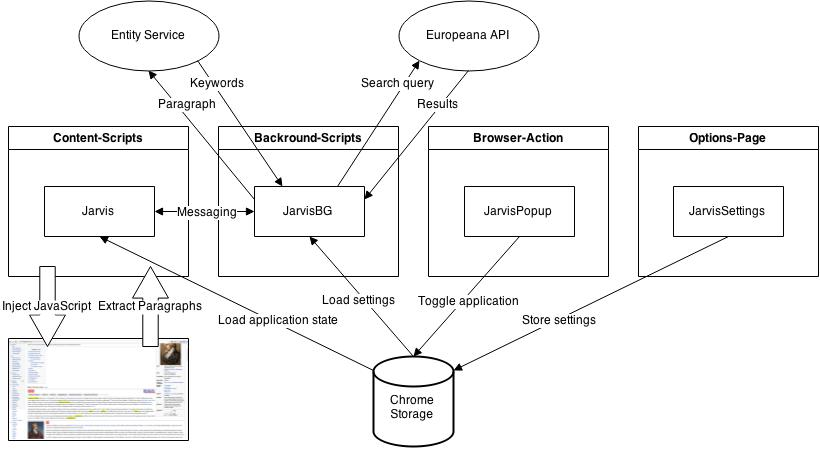
\includegraphics[width=\linewidth]{Bilder/architektur.jpg}
	\captionof{figure}{Kommunikation der AngularJS Komponenten untereinander}
	\label{fig:architektur}
 \end{minipage}
 
 Jarvis ist das Modul, welches in die jeweilige Webseite per JavaScript Injection eingefügt wird. Es extrahiert die Paragraphen aus dem Text und fügt die eigene Direktive in das DOM ein. Die extrahierten Paragraphen werden per Message Passing\footnote{\url{https://developer.chrome.com/extensions/messaging}} an die Background-Skripte weitergegeben. Diese sind zusammengefasst im Modul JarvisBG. 

 Dieses Modul ist zuständig für die Kommunikation mit den REST Endpunkten von Europeana und dem Keyword Service. Im Gegensatz zu Jarvis, welches für jeden offenen Browser-Tab eine eigene Instanz hat, existiert das JarvisBG Modul nur ein mal (wie auch JarvisPopup und JarvisSettings). Jarvis schickt Nachrichten mit dem Namen des angeforderten Services sowie einer Callback-Methode an JarvisBG. Dieses führt die Anfrage aus und übergibt die Ergebnisse der Callback-Methode. Diese sorgt dann dafür, dass die Ergebnisse im Frontend richtig angezeigt werden. 

 JarvisPopup ist das Modul des Popup-Fensters, welches nach klick auf das Icon der Extension rechts des Adressfeldes angezeigt wird. Über das Popup wird der Zustand der Extension im aktuellen Tab gesteuert. Der User kann hier entscheiden, ob das Programm in diesem Tab angezeigt wird oder nicht. Der Zustand wird dann im Chrome Storage\footnote{\url{https://developer.chrome.com/extensions/storage}} gespeichert. Die Wahl für die Speicherung der Anwendungsdaten viel auf den Chrome Storage, da er einige Vorteile gegenüber der localStorage API\footnote{\url{https://developer.mozilla.org/en-US/docs/Web/Guide/API/DOM/Storage\#localStorage}} bietet. Zum einen können die Content-Skripte direkt darauf zugreifen ohne einen Umweg über die Background-Skripte gehen zu müssen. Weiterhin erlaubt Chrome Storage eine automatische Synchronisierung der Inhalte. Dadurch wird Jarvis sofort benachrichtigt, sobald sich der Zustand der Applikation ändert.

 Der Nutzer hat die Möglichkeit, über die Options-Page\footnote{\url{https://developer.chrome.com/extensions/optionsV2}} die verwendeten Services zu konfigurieren. Das dafür zuständige Modul ist JarvisSettings. Es speichert die Einstellungen im Chrome Storage und JarvisBG passt die REST-Anfragen entsprechend an.

 \subsection{Paragraphen-Erkennung}
 \subsection{Paragraphen-Analyse}
  Improving Efficiancy and Accuracy in Multilingual Entity Extraction

 \subsection{Bau der GUIs}
		- > Darf den Benutzer nicht zu sehr ablenken
		- > Ergebnisse müssen in der Nähe ihrer „Quelle“ angezeigt werden (proximity compatibility pricinple)
		- > Benutzer muss klar zwischen Webseite und Augmentation unterscheiden können
		- > buntes, auffälliges Design
		- > Ramping interface: Mehr Benutzerinteraktionen führen zu mehr angezeigten Informationen (Erklärung der Stages) 


 Durch die Chips kann man später auch leicht IQE hinzufügen, zb relevance feedback
 \subsection{Einbindung der REST-Services}
\section{Evaluierung?}
Aufgaben die Benutzer mit EEXCESS Lösen mussten müssen sie jetzt mit Redesign lösen. Vergleich der Ergebnisse?
\section{Future Work}
\label{sec:futureWork}
 \subsection{Verbesserung der Ergebnis-Güte}

  \subsubsection{Speicherung von guten Suchanfragen für jeden Paragraphen}
  \subsubsection{Bewertung von Quellen}

  \subsubsection{Automatic Query Extension}
		Re-examining the Potential Effectivness of Interactive Query Expansion
  Query expansion techniques, e.g. [1,5] aim to improve a user's search by adding new query terms to an existing query. A standart method of performing query expansion is to use relevance information from the user
  All or some of these expansion terms can be added to the query either by the user - interactive query expansion - or by the retrieval system - automatic query expansion.
  argument for IQE is that interactive query expansion gives more control to the user
  We compare the effect of query expansion against no query expansion. how good are different approaches to query expansion? 
  All AQE strategies were more likely on average to improve a query than harm it. All techniques improved at least 50\% of the queries where query expansion could make a difference to retrieval effectivness.
  query dependet strategy not only improves the highest percentage of queries, is most stable, but also gives the highest average precision over the queries, is most effective
  users, especially web searchers, often use very short queries [9]. presenting a list of possible expansion terms is one way to get users to give more information, in the form of query words, to the system.
  people can recognize expansion terms that are semantically related to the informatin for which they are seeking and expand the query using these terms


   \subsubsection{Interactive Query Extension - relevance feedback}
 				Towards Interactive Query Expansion:
  in an era of online retrieval, it is appropriate to offer guidance to users wishing to improve their initial queries. one form of such guidance could be short lists of suggested terms gathered from feedback, nearest neigbhors, and term variants of original query terms
  one method for retrieving more relevant documents is to expand the query terms by using relevance feedback, conflating word stems, and/or adding synonyms form thesaurus. These additional terms allow the query to match documents that contain words which are related to the query, but not actually expressed in it. 
  system should be able to help the user modify the query in order to retrieve more relevant documents
  The size of windows and the patience of the user require that only a reasonable number of terms be displayed
  relevance feedback is an interactive retrieval tool
  with the user selecting terms form a small subset of the terms derived from relevance feedback
  In an interactive situation, the user will select only those terms deemed useful
  it has further been shown that user selection from term vaiants and nearest neighbors of query terms can provide terms for query expansion that improve performance to that comparable with feedback.


  \subsubsection{word sense disambigation (mal schauen)}
	 \cite{budzik2000user}

  \subsubsection{Filtern der Ergebnisse, clustering}
 		(mehr Präzision da Ausbeute bei JITIR nicht so relevant) Clustering\cite{budzik2000user}

 \subsection{Anbindung weiterer Quellen (nur wenn nicht Teil der Implementierung)}
	Automatische Auswahl der richtigen QUelle laut selecting task relevant sources

 \subsection{Portierung der Anwendung auf andere Plattformen}
  \subsubsection{Anpassung der Anwendung für mobile Nutzung}

 \subsection{Beseitigung der Einschränkungen}
 Overlay bauen, whitlistings implementieren

\section{Conclusion}
 \begin{itemize}
 		\item Steigerung der Effektivität und Produktivität von wissenschaftlichem Arbeiten
 		\item Starke Effektivitätssteigerung durch Punkte aus Future Work möglich?
 		\item information management assistants embody a vision of a future in which users hardly ever form a query to request information. when an information need arises, a system like watson has already anticipated it and provided relevant information to the user before she is even able to ask for it (budzik, watson)
 		\item survey suggested that users are relatively dissatisfied with the results of their searching experience. THis makes concrete the claim that systems designed to help useres in their information seeking tasks are needed in the world (budzik, watson)

 		JITIR's can be thought of as automatic ``query free'' search engines (rhodes, using physical context)
 	\end{itemize}

 	Limitations: zB manche seiten werden nicht schön angezeigt

% ----------------------------------------------------------------------------------------------------------
% Literatur
% ----------------------------------------------------------------------------------------------------------
\renewcommand\refname{Quellenverzeichnis}
\bibliographystyle{myalpha}
\bibliography{bibo}
\pagebreak

% ----------------------------------------------------------------------------------------------------------
% Anhang
% ----------------------------------------------------------------------------------------------------------
\pagenumbering{Roman}
\setcounter{page}{1}
\lhead{Anhang \thesection}

\begin{appendix}
\section*{Anhang}
\phantomsection
\addcontentsline{toc}{section}{Anhang}
\addtocontents{toc}{\vspace{-0.5em}}


\subsection*{GUI Screenshots}
\label{app:screenshot}
Unterkategorie, die nicht im Inhaltsverzeichnis auftaucht.

\end{appendix}


\newpage
\thispagestyle{empty}
\begin{center}
	\vspace*{5em}
	\huge\textbf{Erklärung}\\
\end{center}
\vspace{2em}
Hiermit versichere ich, dass ich meine Abschlussarbeit selbständig verfasst und keine anderen als die angegebenen Quellen und Hilfsmittel benutzt habe.

\vspace{4em}
\begin{minipage}{\linewidth}
	\begin{tabular}{p{15em}p{15em}}
		Datum: &  .......................................................\\
		& \centering (Unterschrift)\\
	\end{tabular}
\end{minipage}

\end{document}
